\chapter{序章 はじめに}
NT函館2025のサイドイベントとして企画された「函館機械競馬」。  
"馬"のように見立てたロボット「機械場」が障害物を乗り越え、坂を上り、ゴールを目指す。  
単なるロボコンではなく「競馬」というテーマ性を持たせることで、観客も含めた盛り上がりを実現しました。

函館には有名な函館競馬場があり、毎年多くの客が訪れる函館記念が開催されています。  
これを受けて、NT函館のサブイベントとして、馬を模したロボットがタイムを競い合う「函館機械競馬」を開催することにしました。

\begin{figure}[h]
\centering
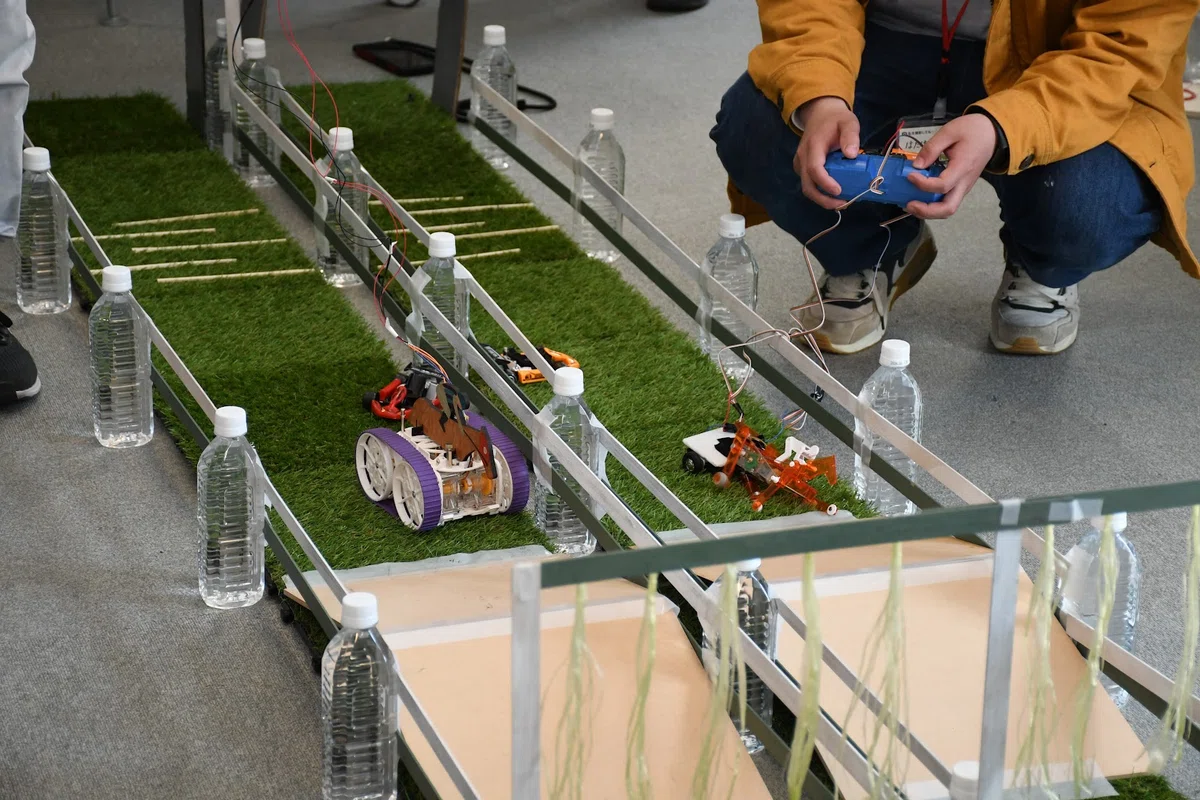
\includegraphics[width=0.7\linewidth]{pages/images/course.png}
\caption{走行中の機械馬たち}
\end{figure}

\chapter{函館機械競馬の思想}
\section{元ネタは調布機械競馬}
函館機械競馬の元ネタは、電気通信大学のサークル「工学研究部」で開催されている「調布機械競馬」です。

調布機械競馬ではロボット同士の干渉(衝突など)・妨害がありのルールでしたが、函館機械競馬では、レーン分けを行いお互いのロボットが干渉しないようにし、自分の機械馬がどれだけ走ってくれるかのみで戦えるようにしています。

また、調布機械競馬ではロボットは4足歩行で自作しないといけないルールでしたが、函館機械競馬ではロボットに馬の要素を取り入れることと、動力源が電気の場合は乾電池しか使用できないというルールで行いました。

\section{参加のしやすさを重視}
これらのルールにした背景としては、函館機械競馬では子供から大人まで気軽に参加できるようにしたかったためです。  
簡単にロボットを作れた方がみんな参加しやすいですからね!

ただし、すべてが簡単すぎても面白くないので、参加条件は簡単にしたもののコースにはいくつかの障害物を設置しました。

\section{競技の概要}
競技はトーナメント形式で行い、1対1のレースで勝敗を決定します。  
ロボットは自律走行でも、コントローラーによる操縦でも構いません。  
各レースで先にゴールしたチームが次の試合に進みます。  
制限時間は90秒とし、その時間内にゴールできなかった場合はその時点で終了となります。

\chapter{コースと仕掛けの舞台裏}
\section{コース設計}
函館機械競馬では、長さ3000mm、幅300mmの直線のコートを2つ並列に並べました。  
コースは300mm×300mmのサイズの人工芝のマットを10枚並べて構成されています。

コースの端には柵を設置し、はじめのマットをスタートエリア、さいごのマットをゴールエリア、その間のマットを走行エリアとしました。  
スタートエリア、ゴールエリアには高さ250mmのゲートを設置しています。

\begin{figure}[h]
\centering
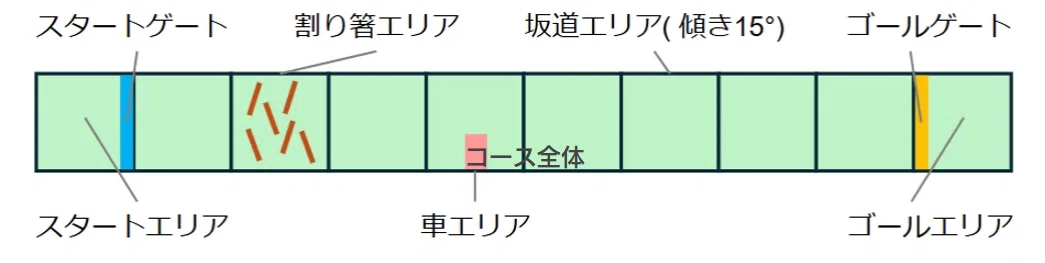
\includegraphics[width=0.7\linewidth]{pages/images/course-layout.png}
\caption{コース全体の様子}
\end{figure}

\section{障害物の配置}
走行エリアにはいくつかの障害物を設置しました。

\begin{itemize}
  \item \textbf{割り箸エリア}:細かい障害物が機械馬の足元を阻む
  \item \textbf{車エリア}:車輪を使った機械馬にとっての試練
  \item \textbf{坂道エリア}:傾き15°の坂道。最大の難関となった
\end{itemize}

特に坂道は木の板でできており、非常に滑りやすく、多くの機械馬がこのセクションで苦戦することになりました。

\section{制作の裏側}
函館機械競馬のコースはほとんどが手作りです!

\subsection{制作協力者たち}
\begin{itemize}
  \item \textbf{Bラボの受講生(機械競馬開催時)のスギ君}  
  スタートゲートの作成、塗装、柵の塗装をめっちゃ手伝ってくれました!
  
  \item \textbf{未来大の工房の職員の方}  
  坂の部分の作成に協力していただきました!
  
  \item \textbf{はこだてIKAの方}  
  前日準備の際に、スタートのゲートやゴールのポールを作ってくれました!
\end{itemize}

様々な方のお力をいただいてコースを完成させることが出来ました!  
本当にありがとうございました!

\chapter{白熱するレース展開}
\section{参加チームたち}
当日は多くのチームが参加し、トーナメント形式で熱戦が繰り広げられました。  
各チームが事前に製作してきた機械馬は、どれも個性的で工夫が凝らされていました。

入賞したチームをご紹介します:
\begin{itemize}
  \item \textbf{Kファクトリー}:安定した走行が光る
  \item \textbf{けすのん}:驚異的なジャンプ機構を搭載
  \item \textbf{公立はこだて未来大学ハードウェアサークル}:粘り強い挑戦
\end{itemize}

\section{函館機械競馬で生まれたドラマ}
\subsection{坂さえ上れればゴール…}
この坂は木の板でできた坂のためとても滑ってしまいます。  
ものすごく頑張って登ろうとしていたのですが、足が滑ってどうしても登れません。  
それでもあきらめずに登ろうとする姿にみんなが応援していました!

\begin{figure}[h]
\centering
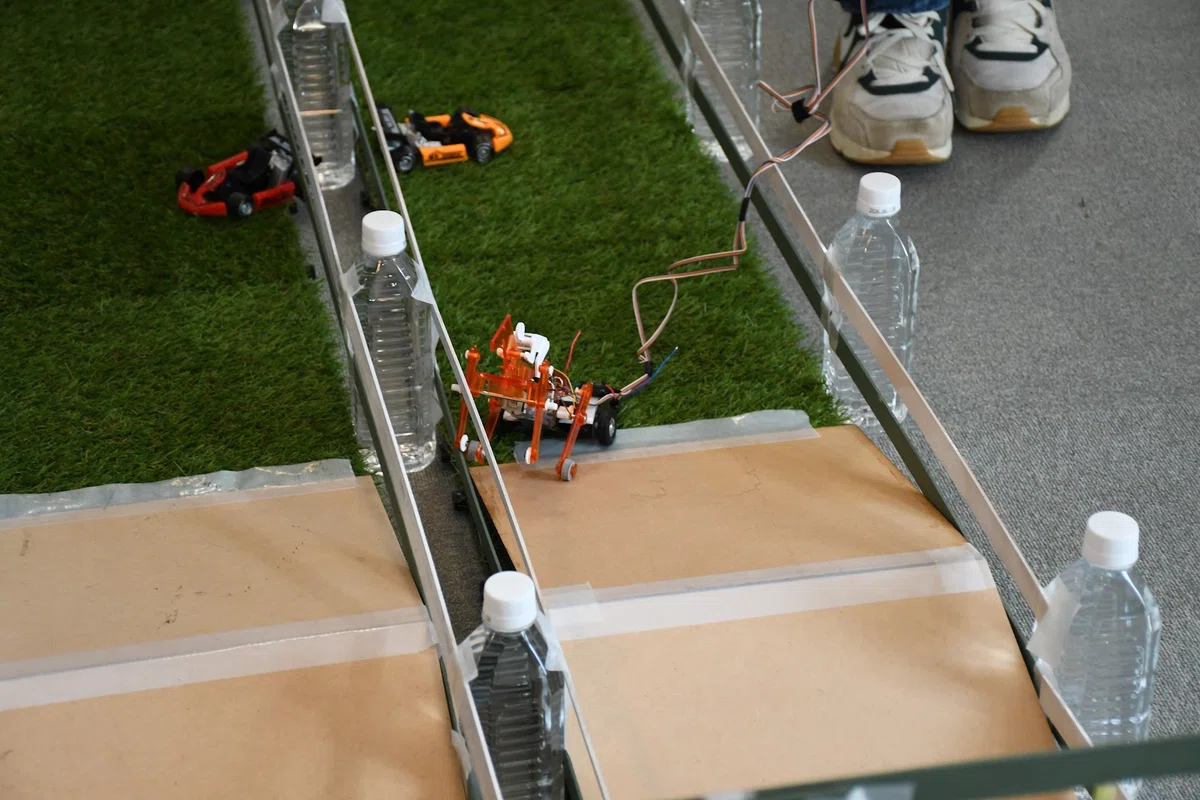
\includegraphics[width=0.7\linewidth]{pages/images/slope.png}
\caption{坂に挑む機械馬。滑りながらも諦めない。}
\end{figure}

\clearpage

\subsection{ひっくり返ってもあきらめるな!}
公立はこだて未来大学ハードウェアサークルの機械馬は、坂の下りの部分まで来てゴール目前!  
そんなところでなんとひっくり返ってしまいました。  
どうにかゴールのゲートまで進め!!とみんなで応援しましたね!

\begin{figure}[h]
\centering
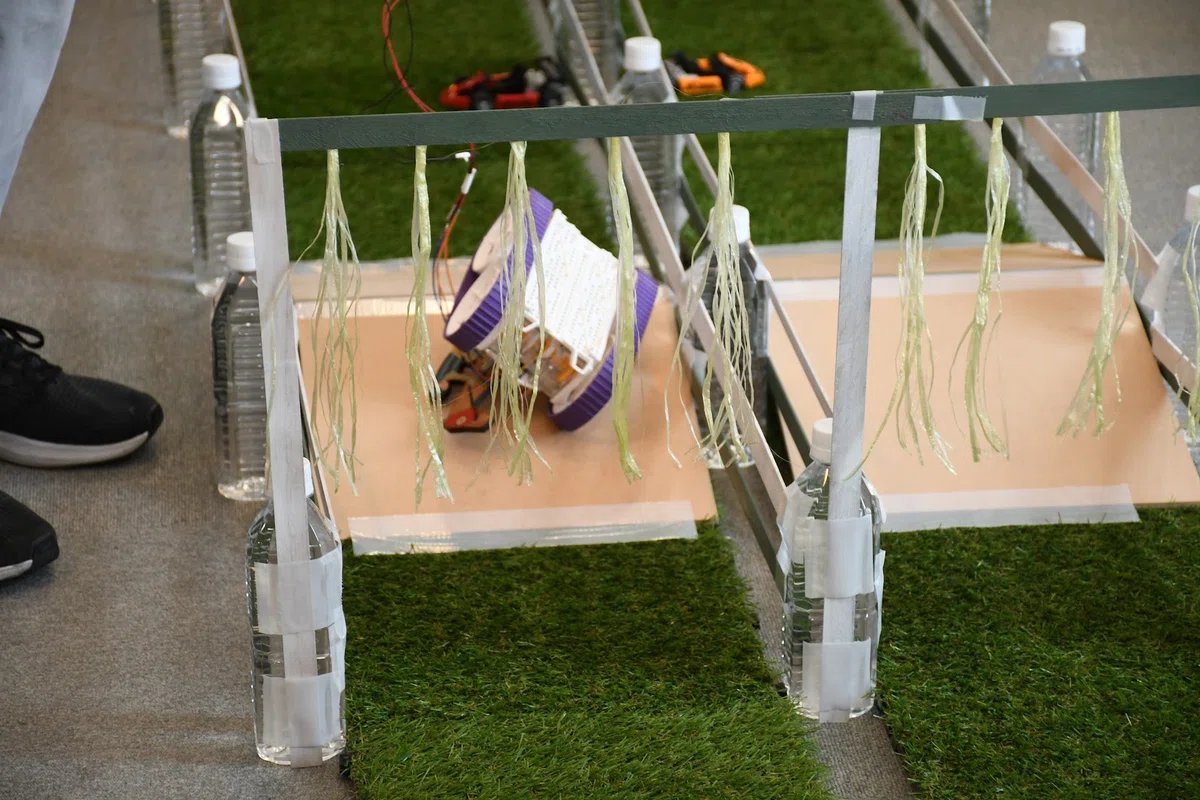
\includegraphics[width=0.7\linewidth]{pages/images/reverse.png}
\caption{ひっくり返ってもあきらめるな!}
\end{figure}

\section{函館機械競馬の見どころ}
\subsection{けすのん「ツツツ・ツツツ」}
スタートと同時に空高く舞い上がりゴールへ向かって一直線!  
全部の障害物をスキップし、今大会最速のゴールを見せてくれました!  
会場は大盛り上がりでしたね!

\begin{figure}[h]
\centering
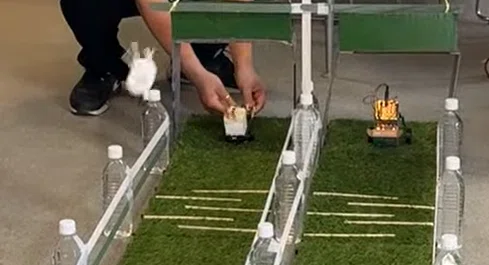
\includegraphics[width=0.7\linewidth]{pages/images/kesumon.png}
\caption{「けすのん」驚愕のジャンプ。会場は歓声に包まれた。}
\end{figure}

\subsection{Kファクトリー「カスガブライアン」}
全試合で超安定した走行を見せてくれました!  
これ、10000回挑戦しても全部成功するんじゃ…っていうくらいの安定感でしたね!  
文句なしの優勝です!

\begin{figure}[h]
\centering
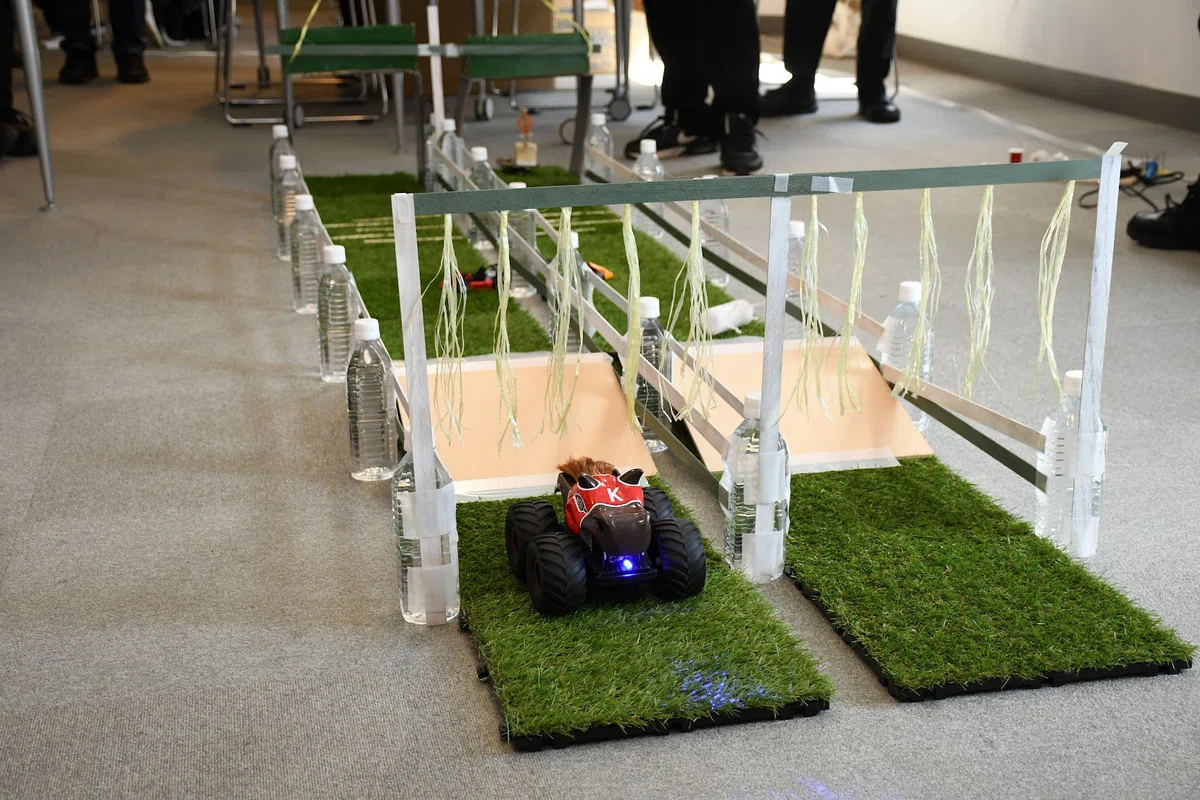
\includegraphics[width=0.7\linewidth]{pages/images/kfactory.png}
\caption{Kファクトリーの安定した走り}
\end{figure}

\chapter{結果発表と特別賞}
\section{最終順位}
トーナメント形式で行われた熱戦の結果、以下のチームが入賞しました。

\begin{enumerate}
  \item \textbf{Kファクトリー}  
  全試合で圧倒的な安定感を見せ、文句なしの優勝。
  
  \item \textbf{けすのん}  
  スタートと同時の驚異的なジャンプで最速ゴールを記録。会場を沸かせた。
  
  \item \textbf{公立はこだて未来大学ハードウェアサークル}  
  困難に立ち向かう姿が観客の心を掴んだ。
\end{enumerate}

\section{特別賞}
タイム以外の魅力を称える特別賞も設けられました。

\begin{itemize}
  \item \textbf{馬かったでしょう賞}:公立はこだて未来大学ハードウェアサークル
  
  \item \textbf{はこだてIKA賞}:NEXT DAY②
\end{itemize}

\begin{figure}[h]
\centering
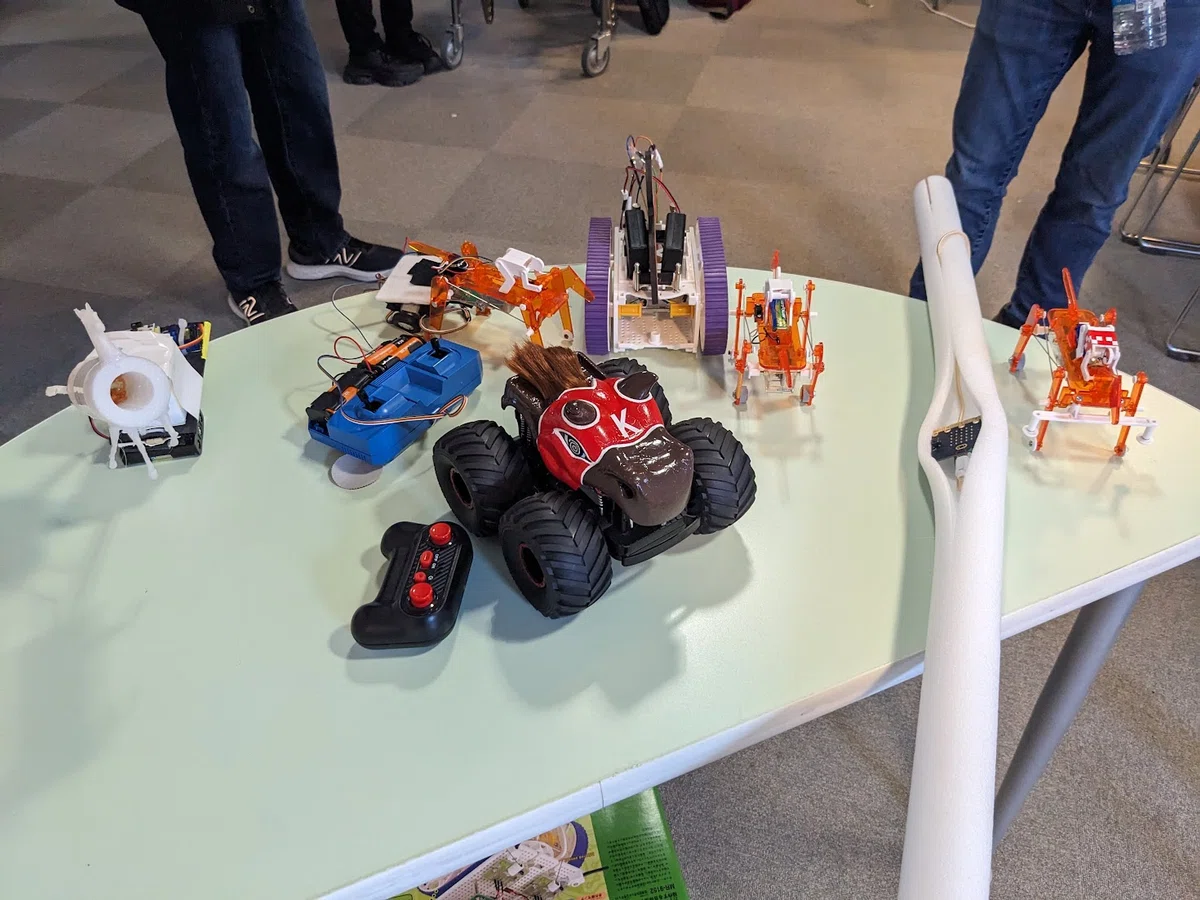
\includegraphics[width=0.7\linewidth]{pages/images/all-robots.png}
\caption{出場してくれた機械馬たち}
\end{figure}

\chapter{運営の振り返り}
\section{よかった点}
今回、多くの方々に参加していただき、非常に盛り上がるイベントとなりました。
様々なドラマが生まれ、ただ競い合うだけでなく、観客も含めた一体感が感じられ、非常に良い雰囲気でイベントを進行できました。

\section{改善点}
一方で、いくつかの改善点も見つかりました。
例えば、自分もそうですが参加者のほとんどはNTの出展者であり、機械競馬に参加している間は展示の対応ができないという問題があります。
もし次回開催するのであれば、前夜祭として開催するなど、展示と競技の両立ができるような工夫が必要だと感じました。

\chapter{あとがきと展望}
今回、準備・運営を手伝ってくださった方々、機械競馬に参加して盛り上げてくださった方々、またNT函館の開催に関係するすべての方々、本当にありがとうございました!

皆様のおかげで函館機械競馬を開催し、大いに盛り上がる会にすることが出来たと思っています!

また、主催者が誰であれ今後ともこういったイベントに参加していただき、函館を盛り上げていっていただけると幸いです!

函館機械競馬が、函館の新たな風物詩として育っていくことを願っています。